\documentclass[a4paper, 12pt]{article}

\newcommand\tab[1][.6cm]{\hspace*{#1}}
\usepackage[portuges]{babel}
\usepackage[utf8]{inputenc}
\usepackage{amsmath}
\usepackage{mathtools}
\usepackage{indentfirst}
\usepackage{graphicx}
\usepackage{multicol,lipsum}
\usepackage{blindtext}
\usepackage{verbatim}
\usepackage{textcomp}
\usepackage{hyperref}
\usepackage{float}
\usepackage{url}

\begin{document}
%\maketitle

\begin{titlepage}
	\begin{center}
	
	\begin{figure}[ht]
    \centering
    
\includegraphics[width=.44\textwidth]{Images/LogoUFSJ.PNG}
    \label{fig:Capturar.PNG}
    \end{figure}

    	\Huge{Universidade Federal São João del Rei}\\
		\Large{Curso de Ciência da Computação}\\ 

        \vspace{110pt}
        \textbf{\LARGE{
        \\
        \\
        \\
        Exercícios Avaliativos\\
        \vspace{0.5cm}
        \Large{Introdução à Modelagem Computacional}
        \\
        \\
        \\
        }}
        
		\title{{\large{Título}}}
		\vspace{2.5cm}
	\end{center}
	    
    \begin{flushleft}
		\begin{tabbing}
		\\
		\\
		\\	
		\large{Discente: Julio Cesar da Silva Rodrigues}\\
	    \\
		\large{Docente: Alexandre Bittencourt Pigozzo}\\
	    \end{tabbing}
    \end{flushleft}
	\vspace{1cm}
	
	\begin{center}
		\vspace{\fill}
			Maio\\
		    2023
	\end{center}
\end{titlepage}

\section*{Exercício 1}

O modelo construído utilizando a ferramenta \emph{Insight Maker} que representa a ocorrência das reações é exibido na Figura \ref{fig:exampleFig1}.

\begin{figure}[H]
    \centering
    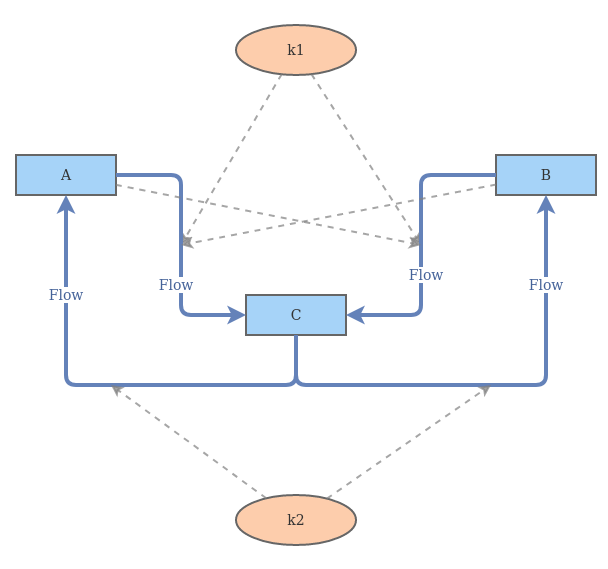
\includegraphics[width=1\textwidth]{Images/Exercise 1/model.png}
    \caption{Modelo de Reações Químicas}
    \label{fig:exampleFig1}
\end{figure}

Foi criado um conjunto de \emph{stocks} representando as moléculas hipotéticas que correspondem as populações A, B e C (e seus níveis de concentração).

Foram criados dois fluxos direcionados para C, e ambos possuem a mesma modelagem do número de reações, multiplicando a taxa \emph{\(k_1\)} pelas concentrações de A e B ao longo do tempo, produzindo C.

\begin{align*}
    \frac{dA}{dt} = k_1 \cdot A \cdot B \hspace{1cm}
    \frac{dB}{dt} = k_1 \cdot A \cdot B
\end{align*}

De forma semelhante, foram criados dois fluxos para representar a reação de volta, desta vez com uma taxa \(k_2\) com que a concentração de moléculas de C "derivam" A e B, aumentando suas concentrações.
\begin{align*}
    \frac{dC}{dt} = k_2 \cdot C
\end{align*}

Uma simulação\(^*\) inicial foi realizada (Figura \ref{fig:exampleFig2}), utilizando as condições iniciais à seguir:

\begin{itemize}
    \item \(A = 2\)
    \item \(B = 1\)
    \item \(C = 0\)
    \item \(k_1 = 0.1\)
    \item \(k_2 = 0.05\)
\end{itemize}

\begin{figure}[H]
    \centering
    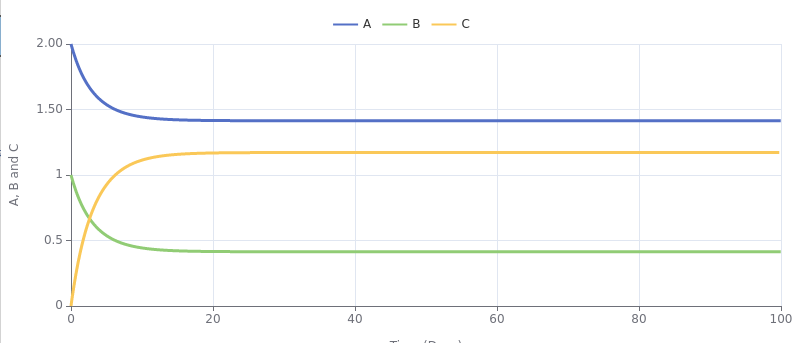
\includegraphics[width=1\textwidth]{Images/Exercise 1/vanilla.png}
    \caption{Reações Químicas ao Longo do Tempo}
    \label{fig:exampleFig2}
\end{figure}

\noindent * Todas as simulações deste exercício foram realizadas com passo de tempo 0,01 e mensurado em dias.

\subsection*{Alterando Parâmetros, Condições Iniciais e Análises}

Para o parâmetro \(k_1\), foi observado que elevações em seu valor implicam no aumento da concentração de C em relação as concentrações de A e B, que se mostram inferiores como é mostrado na Figura \ref{fig:exampleFig3}. As condições iniciais da simulação são detalhadas à seguir:

\begin{itemize}
    \item \(A = 2\)
    \item \(B = 1\)
    \item \(C = 0\)
    \item \(k_1 = 1\)
    \item \(k_2 = 0.05\)
\end{itemize}

\begin{figure}[H]
    \centering
    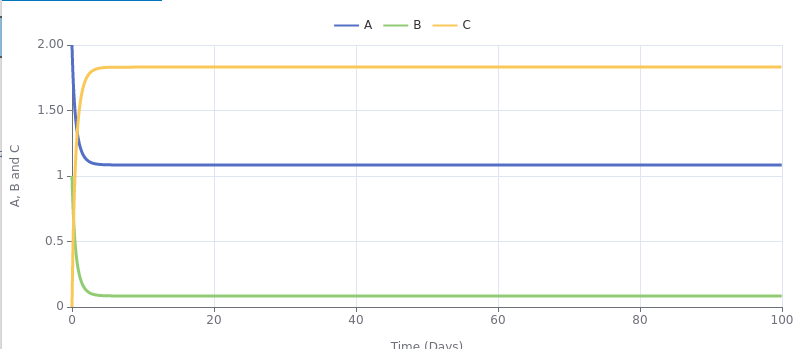
\includegraphics[width=1\textwidth]{Images/Exercise 1/k1.png}
    \caption{Reações Químicas ao Longo do Tempo Variando \(k_1\)}
    \label{fig:exampleFig3}
\end{figure}

Em contrapartida, atribuindo valores muito baixos para \(k_1\) produzem um efeito inverso, com C apresentando uma concentração menor em relação as concentrações de A e B ao longo do tempo na simulação.

Para o parâmetro \(k_2\), foi observado que elevações em seu valor implicam em pouco decréscimo nas concentrações de A e B, enquanto o crescimento de C se mostra relativamente discreto, com concentração final inferior as de A e B como é mostrado na Figura \ref{fig:exampleFig4}. As condições iniciais da simulação são detalhadas à seguir:

\pagebreak

\begin{itemize}
    \item \(A = 2\)
    \item \(B = 1\)
    \item \(C = 0\)
    \item \(k_1 = 0.1\)
    \item \(k_2 = 0.5\)
\end{itemize}

\begin{figure}[H]
    \centering
    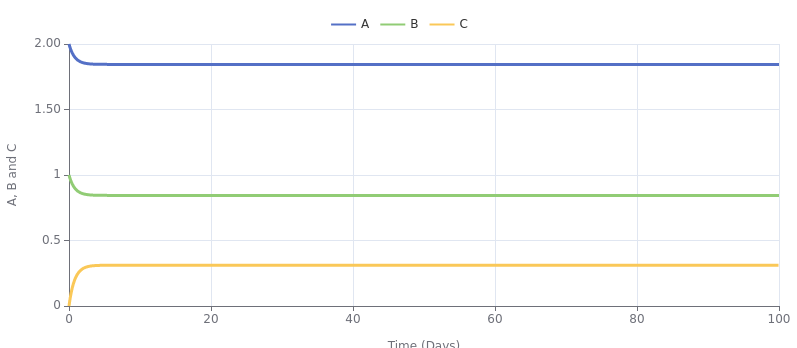
\includegraphics[width=1\textwidth]{Images/Exercise 1/k2.png}
    \caption{Reações Químicas ao Longo do Tempo Variando \(k_2\)}
    \label{fig:exampleFig4}
\end{figure}

Além disso, a atribuição de valores muito baixos para \(k_2\) produzem um efeito ainda mais discrepante, com C apresentando uma crescimento quase desprezível em relação as concentrações de A e B ao longo do tempo na simulação.

Em resumo, para as condições iniciais em que as concentrações de A e B são superiores a de C, valores extremos de \(k_1\) aceleram ou inibem o aumento da concentração de C e decréscimo nas concentrações de A e B. Valores extremos de \(k_2\) tendem a estagnar rapidamente as concentrações de A e B ao longo do tempo e inibir proporcionalmente a síntese de C.

Por fim, foi realizada uma última simulação (Figura \ref{fig:exampleFig5}), desta vez com a concentração inicial de C superior às concentrações de A e B, sem alterar as taxas iniciais de \(k_1\) e \(k_2\). O resultado obtido foi o esperado, com a concentração de C apresentando decréscimo, e as concentrações de A e B apresentando crescimento, uma situação inversa à aquela observada na primeira simulação. As condições iniciais da simulação são detalhadas à seguir:

\begin{itemize}
    \item \(A = 1\)
    \item \(B = 0\)
    \item \(C = 3\)
    \item \(k_1 = 0.1\)
    \item \(k_2 = 0.05\)
\end{itemize}

\begin{figure}[H]
    \centering
    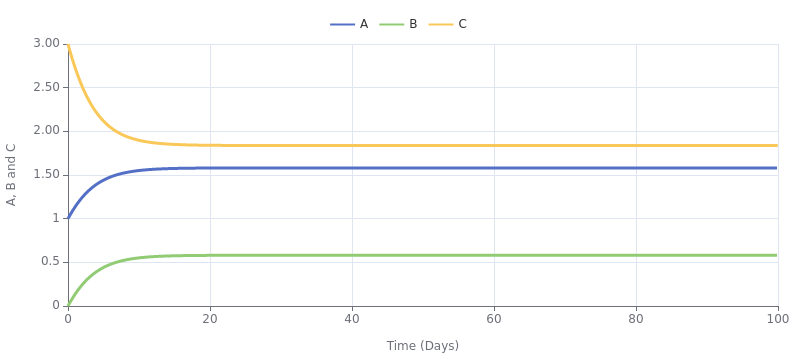
\includegraphics[width=1\textwidth]{Images/Exercise 1/c.png}
    \caption{Impacto das Condições Iniciais na Simulação}
    \label{fig:exampleFig5}
\end{figure}

\section*{Exercício 2}

Para a modelagem de cada uma das EDOs, assume-se como significado de cada variável:

\begin{itemize}
    \item \(A\): Concentração de moléculas do tipo A;
    \item \(B\): Concentração de moléculas do tipo B;
    \item \(C\): Concentração de moléculas do tipo C;
    \item \(k_1\): Probababilidade da reação (síntese) entre duas moléculas quaisquer A e B para produzir C (A + B $\xRightarrow{k_1}$ C);
    \item \(k_2\): Probababilidade da reação (decomposição) de uma molécula qualquer C para produzir A e B (C $\xRightarrow{k_2}$ A + B).
\end{itemize}

\subsection*{Reação com A e B}
\begin{align*}
    \frac{dA}{dt} & = - k_1 \cdot A \cdot B + k_2 \cdot C\\
    \\ \frac{dB}{dt} & = - k_1 \cdot A \cdot B + k_2 \cdot C
\end{align*}

Como apenas existe uma única reação entre A e B de forma conjunta, é utilizada a mesma EDO para modelar suas concentrações ao longo do tempo. O termo \(-k_{1}AB\) representa o decréscimo (sinal negativo) nas concentrações de A e B com uma taxa \(k_1\), conforme a ocorrência das reações. Já o termo \(k_{2}C\) ,representa o aumento (sinal positivo) na concentração de moléculas do tipo C, com uma taxa \(k_2\) à medida que as reações ocorrem, com A e B derivando C (reação de síntese).

\subsection*{Reação com C}
\begin{align*}
    \frac{dC}{dt} & = k_1 \cdot A \cdot B - k_2 \cdot C
\end{align*}

O termo \textbf{\(k_{1}AB\)} representa o aumento (sinal positivo) nas concentrações de A e B com uma taxa \(k_1\), conforme a ocorrência das reações. Já o termo \(-k_{2}C\), representa o decréscimo (sinal negativo) na concentração de moléculas do tipo C, com uma taxa \(k_2\) à medida que as reações ocorrem, com C decompondo-se em A e B (reação de decomposição).

\subsection*{Resultados}

Por fim, foram realizadas simulações utilizando os mesmos parâmetros explorados no modelo sintetizado na plataforma \emph{Insight Maker} para testar o funcionamento correto, e principalmente, a concordância entre resultados para investigar possíveis incoerências. Os resultados obtidos foram extremamente parecidos com aqueles sumarizados pelos gráficos apresentados nas Figuras \ref{fig:exampleFig2}, \ref{fig:exampleFig3}, \ref{fig:exampleFig4} e \ref{fig:exampleFig5} (inclusive as análises).

Para efeitos de comparação e checagens, os resultados obtidos com o modelo desenvolvido em linguagem \emph{Python} são exibidos nas Figuras \ref{fig:exampleFig6}, \ref{fig:exampleFig7}, \ref{fig:exampleFig8} e \ref{fig:exampleFig9}:

\begin{figure}[H]
    \centering
    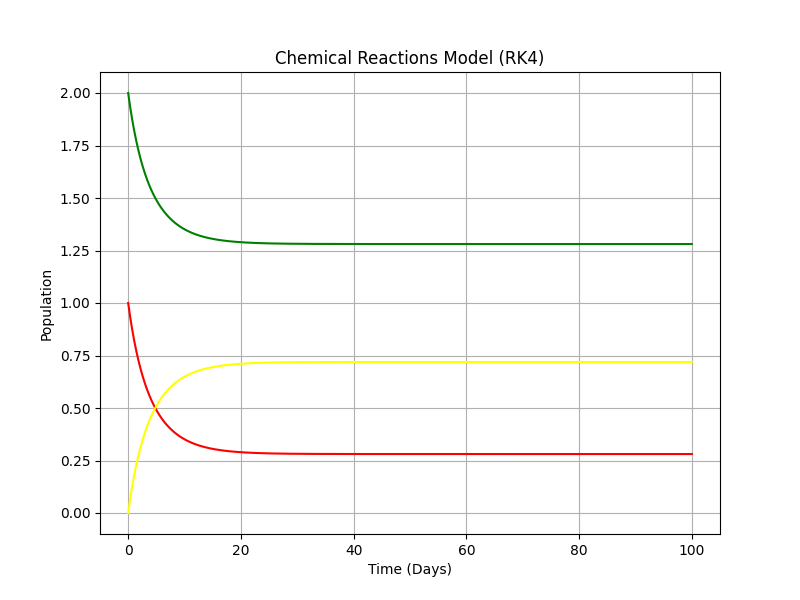
\includegraphics[width=0.88\textwidth]{Images/Exercise 2/vanilla.png}
    \caption{Reações Químicas ao Longo do Tempo}
    \label{fig:exampleFig6}
\end{figure}

\begin{figure}[H]
    \centering
    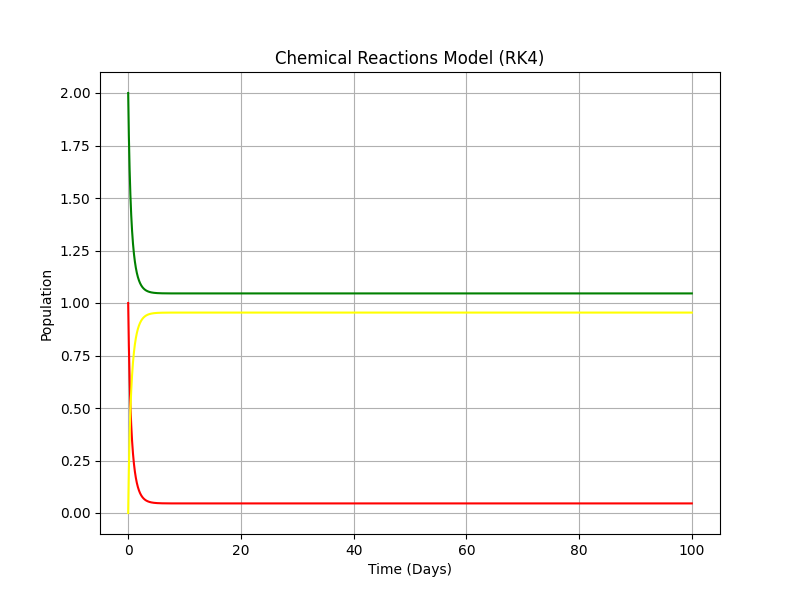
\includegraphics[width=0.88\textwidth]{Images/Exercise 2/k1.png}
    \caption{Reações Químicas ao Longo do Tempo Variando \(k_1\)}
    \label{fig:exampleFig7}
\end{figure}

\begin{figure}[H]
    \centering
    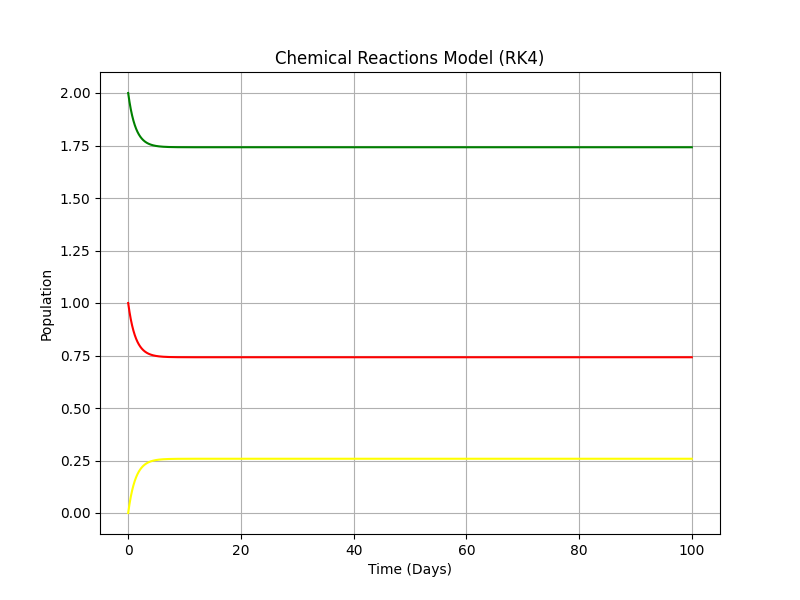
\includegraphics[width=0.88\textwidth]{Images/Exercise 2/k2.png}
    \caption{Reações Químicas ao Longo do Tempo Variando \(k_2\)}
    \label{fig:exampleFig8}
\end{figure}

\begin{figure}[H]
    \centering
    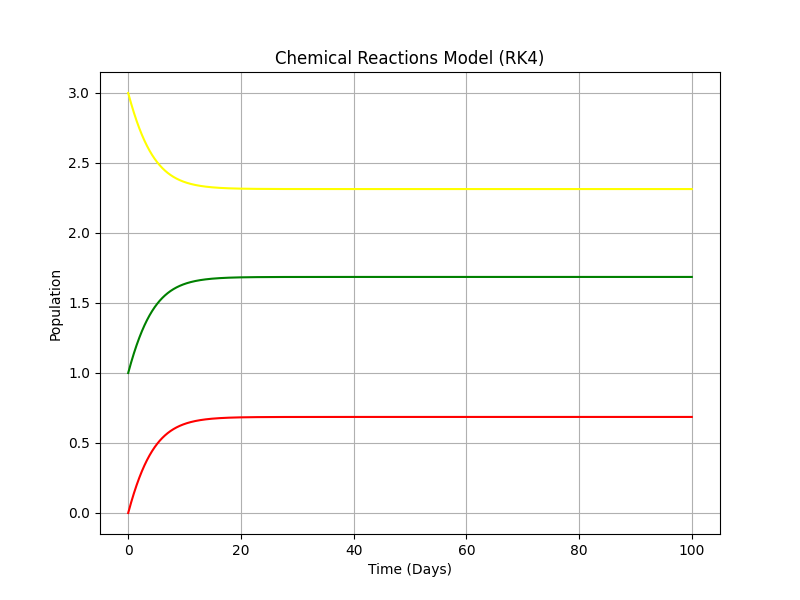
\includegraphics[width=0.88\textwidth]{Images/Exercise 2/ic.png}
    \caption{Impacto das Condições Iniciais na Simulação}
    \label{fig:exampleFig9}
\end{figure}

\section*{Exercício 3}

\subsection*{EDOs}

\begin{itemize}
    \item Produto P
    \begin{align*}
        \frac{dP}{dt} & = k_3 \cdot ES
    \end{align*}
    \item Substância I
    \begin{align*}
        \frac{dI}{dt} & = - (k_4 \cdot E \cdot I) + (k_5 \cdot EI)
    \end{align*}
    \item Substrato S
    \begin{align*}
        \frac{dS}{dt} & = - (k_1 \cdot S \cdot E) + (k_2 \cdot ES)
    \end{align*}
    \item Complexo Temporário ES
    \begin{align*}
        \frac{dES}{dt} & = k_1 \cdot E \cdot S - k_2 \cdot ES - k_3 \cdot ES\\
        & = (k_1 \cdot E \cdot S) - (ES \cdot(k_2 + k_3))
    \end{align*}
    \item Complexo Temporátio EI
    \begin{align*}
        \frac{dEI}{dt} & = (k_4 \cdot E \cdot I) - (k_5 \cdot EI)
    \end{align*}
    \item Enzima E
    \begin{align*}
        \frac{dE}{dt} & = k_2 \cdot ES + k_3 \cdot ES + k_5 \cdot EI - k_1 \cdot S \cdot E - k_4 \cdot E \cdot I\\
        & = (ES \cdot (k_2 + k_3)) + (k_5 \cdot EI) - (k_1 \cdot S \cdot E) - (k_4 \cdot E \cdot I)
    \end{align*}
\end{itemize}

\subsection*{Resultados Iniciais}

Nesta subseção, serão apresentados alguns dos resultados obtidos nos testes e simulações realizadas. É importante citar de antemão, que os valores passo de tempo (\(dt\)) e o tempo total de simulação (\(t_{final}\)), foram sempre constantes (0,1 e 100). Além disto, o método utilizado na resolução foi o \emph{Runge-Kutta} de 4ª ordem.

\subsubsection*{Primeira Simulação}

No primeiro teste realizado, os parâmetros e condições iniciais foram fixados com o mesmo valor. O resultado pode ser observado na Figura \ref{fig:exampleFig10}, cuja execução se deu com os seguintes valores:

\begin{itemize}
    \item \(E = S = I = P = ES = EI = 20\);
    \item \(k_1 = k_2 = k_3 = k_4 = k_5 = 0,1\).
\end{itemize}

\vspace*{-1cm}

\begin{figure}[H]
    \centering
    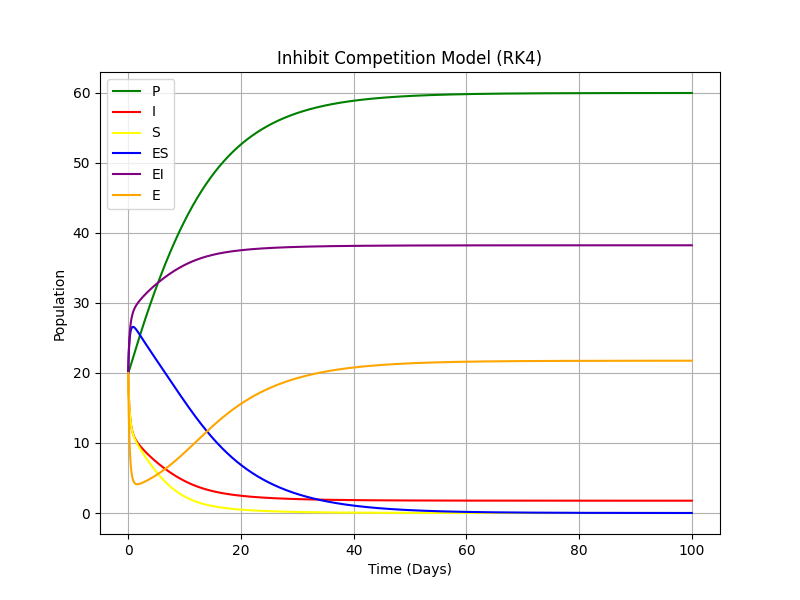
\includegraphics[width=1\textwidth]{Images/Exercise 3/same.png}
    \vspace*{-1cm}
    \caption{Impacto de parâmetros iguais na simulação}
    \label{fig:exampleFig10}
\end{figure}

Embora os valores das condições iniciais e taxas sejam exatamente os mesmos entre si, podemos observar alguns comportamentos interessantes do modelo. A variação das populações alcança a estabilidade por volta de \(t = 40\), e apenas duas populações apresentam crescimento ao final da simulação, em relação às condições iniciais.

Nos primeiros instantes de tempo, \emph{E} e \emph{S} reagem rapidamente formando \emph{ES}, cuja população cresce exponencialmente brevemente (e as populações de \emph{E} e \emph{S} diminuem). Logo após, esse crescimento não só estagna, como começa a decrescer exponencialmente devido à reação de volta (\(ES \rightarrow E + S\)) e a reação de ida (\(ES \rightarrow E + P\)). Como não existe reação de volta entre \emph{E}, \emph{P} e \emph{ES} (\(E + P \rightarrow ES\)), a população de \emph{E} volta a crescer, e \emph{ES} tende à zero.

Já na segunda reação cinética (\(E + I \leftrightarrow EI\)), como a enzima \emph{E} participa na síntese e decomposição em todas as reações, esta descresce rapidamente, para então crescer e se estabilizar novamente. Neste momento, as concentração de \emph{ES} e \emph{S} já estagnaram (tendem à zero), assim como a população de I. Por isto, \emph{EI} cresce em função logarítimica até se estagnar em \(t = 20\).

\subsubsection*{Segunda Simulação}

No segundo teste realizado, as taxas e condições iniciais foram subitamente alteradas. As reações de síntese de \emph{S}, \emph{E} e \emph{P} foram suprimidas (\(ES \rightarrow S + E\) e \(ES \rightarrow E + P\)), fixando as taxas \(k_2\) e \(k_3\) como nulas. O resultado pode ser observado na Figura \ref{fig:exampleFig11}, cuja execução se deu com os seguintes valores:

\begin{itemize}
    \item \(E = S = I = EI = 10\) \hspace{0.1cm}\textbar\hspace{0.1cm} \(P = 13\) \hspace{0.1cm}\textbar\hspace{0.1cm} \(ES = 15\);
    \item \(k_2 = k_3 = 0\) \hspace{0.1cm}\textbar\hspace{0.1cm} \(k_4 = k_5 = 0,01\) \hspace{0.1cm}\textbar\hspace{0.1cm} \(k_1 = 0,2\);
\end{itemize}

\begin{figure}[H]
    \centering
    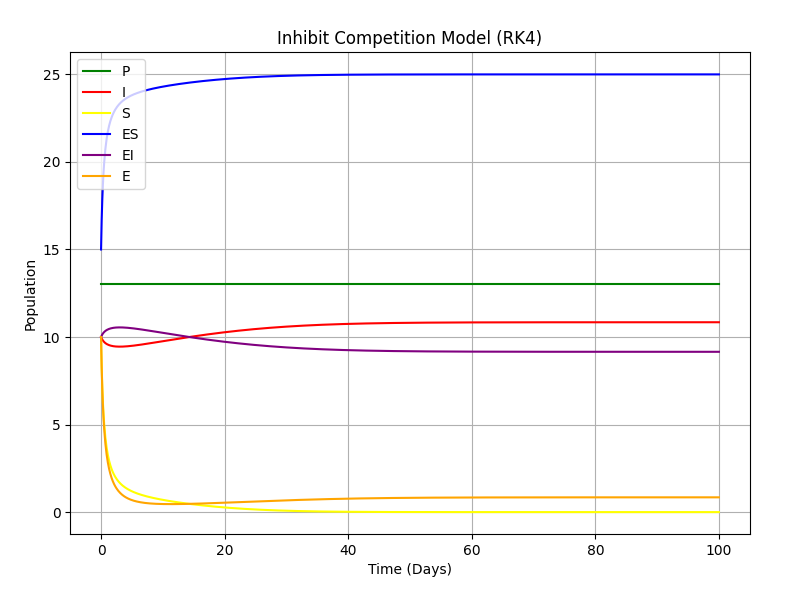
\includegraphics[width=1\textwidth]{Images/Exercise 3/supressed.png}
    \vspace*{-1cm}
    \caption{Variações bruscas nos parâmetros na simulação}
    \label{fig:exampleFig11}
\end{figure}

Como \(k_3\) é igual à zero, a reação de síntese \{\(ES \rightarrow E + P\)\} não ocorre. Logo, a população de \emph{P} permanece inalterada durante toda a simulação. A não ocorrência da reação \{\(ES \rightarrow S + E\)\}, com \(k_2\) igual à zero, impede qualquer decomposição do complexo ES em qualquer substância. Logo, o crescimento da mesma é dado por uma função inicialmente exponencial, que se estagna a partir de \(t = 20\).

Quanto às outras reações do sistema, a população de \emph{S} tende à zero rapidamente devido as reações com \emph{E} para síntese de \emph{ES}, e as reações com \emph{I} para a produção de \emph{EI}. Como \(k_2\) e \(k_3\) são iguais à zero, e as taxas \(k_4\) e \(k_5\) são muito baixas comparadas à \(k_1\), as populações de \emph{E} e \emph{S} não possuem "chances para se recompor" em relação às condições iniciais. Por fim, com o esgotamento rápido da enzima \emph{E} na síntese de \emph{ES}, \emph{EI} e \emph{I} sofrem pouca variação

\subsubsection*{Terceira Simulação}

No terceiro teste realizado, as taxas e condições iniciais foram subitamente alteradas novamente. A reação de síntese de \emph{ES} foi suprimidas (\(S + E \rightarrow ES\)), fixando a taxa \(k_1\) como nula. O resultado pode ser observado na Figura \ref{fig:exampleFig12}, cuja execução se deu com os seguintes valores:

\begin{itemize}
    \item \(E = I = EI = 15\) \hspace{0.1cm}\textbar\hspace{0.1cm} \(P = 0\) \hspace{0.1cm}\textbar\hspace{0.1cm} \(ES = 20\) \hspace{0.1cm}\textbar\hspace{0.1cm} \(S = 5\);
    \item \(k_2 = k_3 = 0,1\) \hspace{0.1cm}\textbar\hspace{0.1cm} \(k_4 = 0,01\) \hspace{0.1cm}\textbar\hspace{0.1cm} \(k_1 = 0\) \hspace{0.1cm}\textbar\hspace{0.1cm} \(k_5 = 0,4\);
\end{itemize}

\begin{figure}[H]
    \centering
    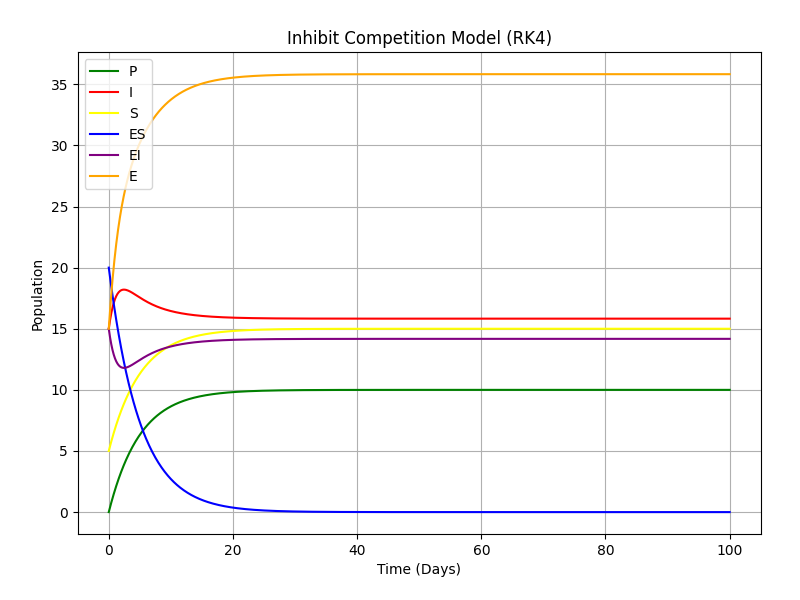
\includegraphics[width=1\textwidth]{Images/Exercise 3/ei.png}
    \vspace*{-1cm}
    \caption{Variações bruscas nos parâmetros na simulação}
    \label{fig:exampleFig12}
\end{figure}

Ao contrário da segunda simulação, como \(k_1\) é igual à zero, a reação de síntese \{\(S + E \rightarrow  ES\)\} não ocorre. Logo, a população de \emph{ES} tende à zero rapidamente. Em contrapartida, as taxas \(k_2\) e \(k_3\) são diferentes de zero, sintetizando \emph{S}, \emph{E} e \emph{P} desde que a população inicial de \emph{ES} seja diferente de zero.

Como a taxa \(k_4\) é relativamente baixa, ocorrem poucas reações de síntese de \emph{EI}, o que mantém a população da mesma e de \emph{I} com pouca variação no início da simulação, e estáveis a partir de \(t = 20\). Outra consequência disto, é de que as populações de \emph{E}, \emph{S} e \emph{P} crescem exponencialmente no começo e se estagnam também em \(t = 20\). Isto é auxiliado pelo fato de que, a taxa \(k_5\) se apresenta bastante alta, sintetizando um grande volume de enzimas \emph{E} e substratos \emph{S} a partir da decomposição dos complexos temporários \emph{ES} e \emph{EI}.

Por fim, existem certas constantes neste modelo. Supondo que não existam condições extremas, como taxas iguais à zero, a produção de um complexo, seja ele \emph{EI} ou \emph{ES}, inibe a produção do segundo. Por isto, a concavidade das curvas dos mesmos tendem à ser opostas. Além disto, como \emph{P} não possui reação de decomposição em nenhuma substância, o crescimento da população do mesmo sempre ocorre na maioria das simulações, supondo novamente que uma ou mais taxas e populações seja diferente de zero. 
 
\section*{Exercício 4}

\subsection*{Letra A}

\begin{itemize}
    \item \textbf{I}\\
    A melhor solução obtida foi \{0,12596218 \textbar\hspace{0.1cm} 0,01300145 \textbar\hspace{0.1cm} 0,85244477\}, com erro associado de aproximadamente 0,26.
    \item \textbf{II}
    \begin{figure}[H]
        \centering
        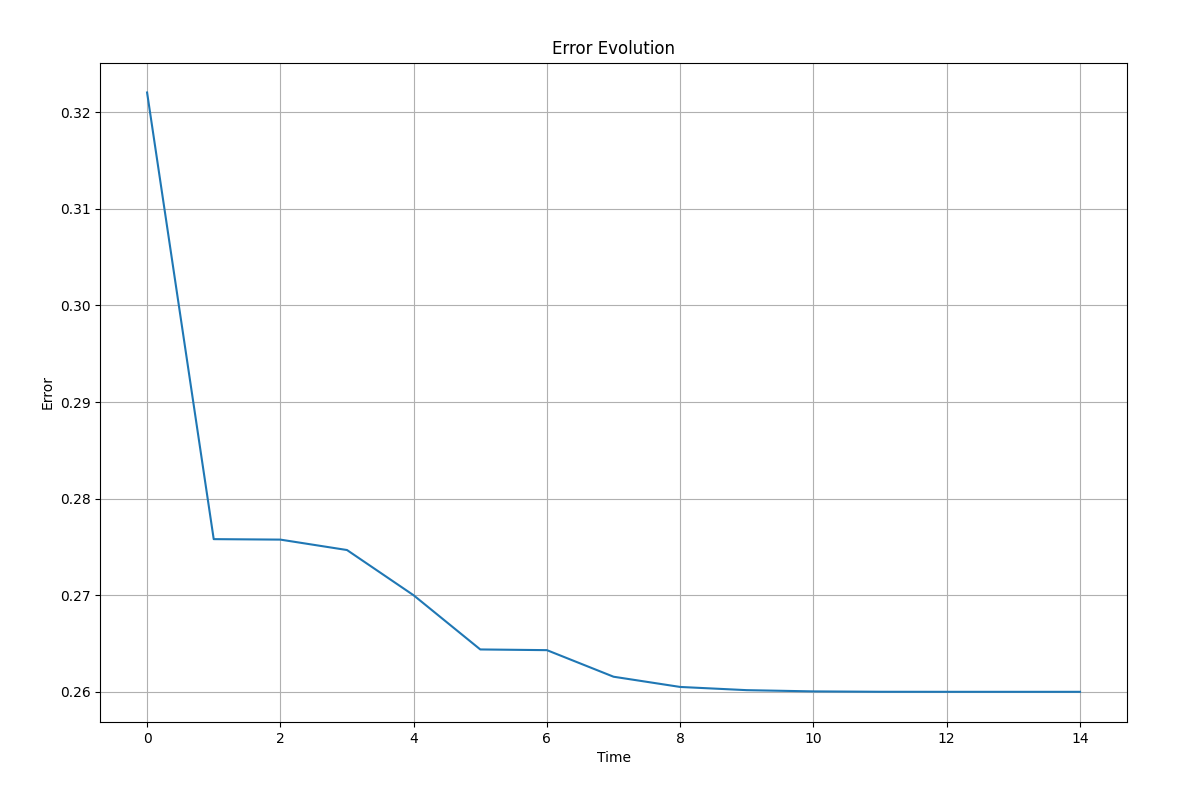
\includegraphics[width=1\textwidth]{Images/Exercise 4/de_error.png}
        \vspace*{-1cm}
        \caption{Evolução do Erro (Evolução Diferencial)}
        \label{fig:exampleFig13}
    \end{figure}
    \item \textbf{III}
    \item \textbf{IV}
\end{itemize}

\pagebreak

\subsection*{Letra B}

\begin{itemize}
    \item \textbf{I}\\
    A melhor solução obtida foi \{0,665573 \textbar\hspace{0.1cm} 0,330446 \textbar\hspace{0.1cm} 0,151489\}, com erro associado de aproximadamente 0,29.
    \item \textbf{II}
    \begin{figure}[H]
        \centering
        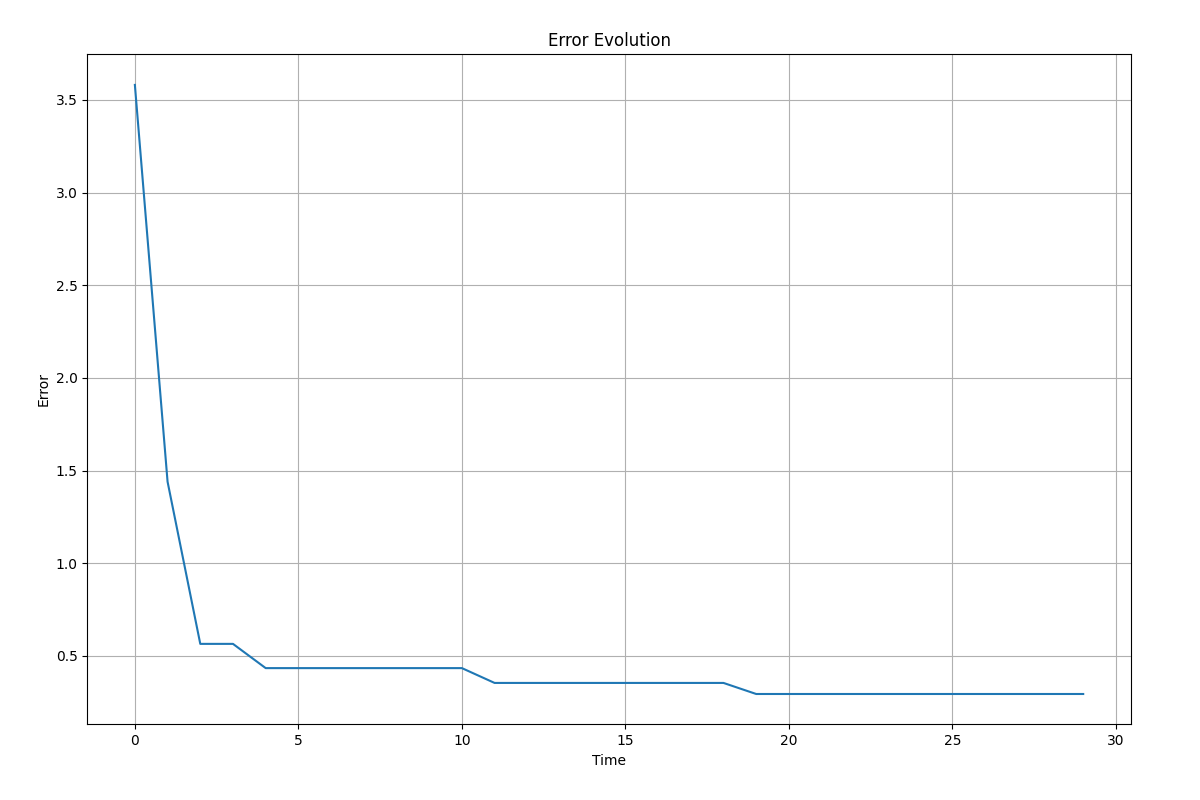
\includegraphics[width=1\textwidth]{Images/Exercise 4/ga_error.png}
        \vspace*{-1cm}
        \caption{Evolução do Erro (Algoritmo Genético)}
        \label{fig:exampleFig14}
    \end{figure}
    \item \textbf{III}
    \item \textbf{IV}
\end{itemize}

Embora os parâmetros utilizados nos algoritmos tenham sido os mesmos, o algoritmo de Evolução Diferencial apresentou o menor erro.

\section*{Exercício 5}

\subsection*{1º Cenário}

Neste primeiro cenário, foram realizados dois testes, cada um executando cinco simulações distintas. Os resultados são sumarizados nas Figuras \ref{fig:exampleFig15}, \ref{fig:exampleFig16} e \ref{fig:exampleFig17}, e \ref{fig:exampleFig18}, \ref{fig:exampleFig19} e \ref{fig:exampleFig20}, respectivamente.

\pagebreak

\begin{itemize}
    \item Primeiro Teste
    \begin{figure}[H]
        \centering
        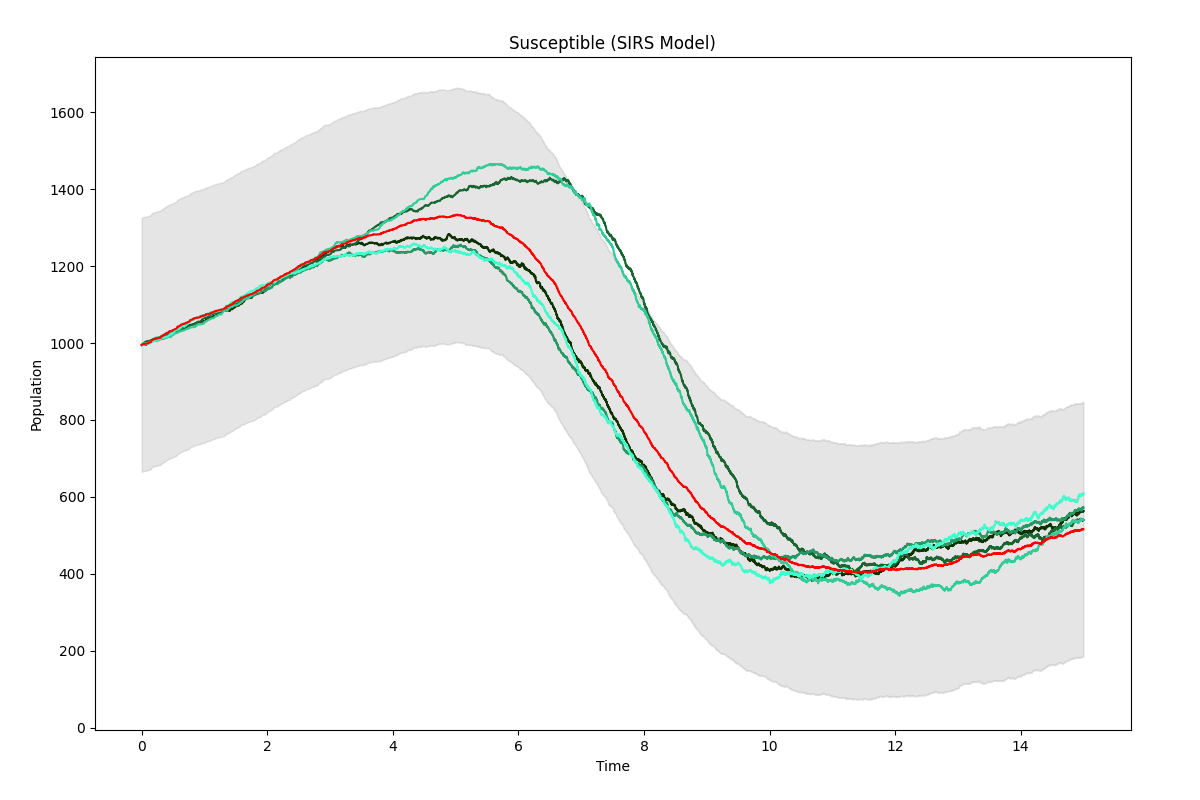
\includegraphics[width=1\textwidth]{Images/Exercise 5/Scenario 1/s1a.png}
        \vspace*{-1cm}
        \caption{Suscetíveis}
        \label{fig:exampleFig15}
    \end{figure}
    
    \begin{figure}[H]
        \centering
        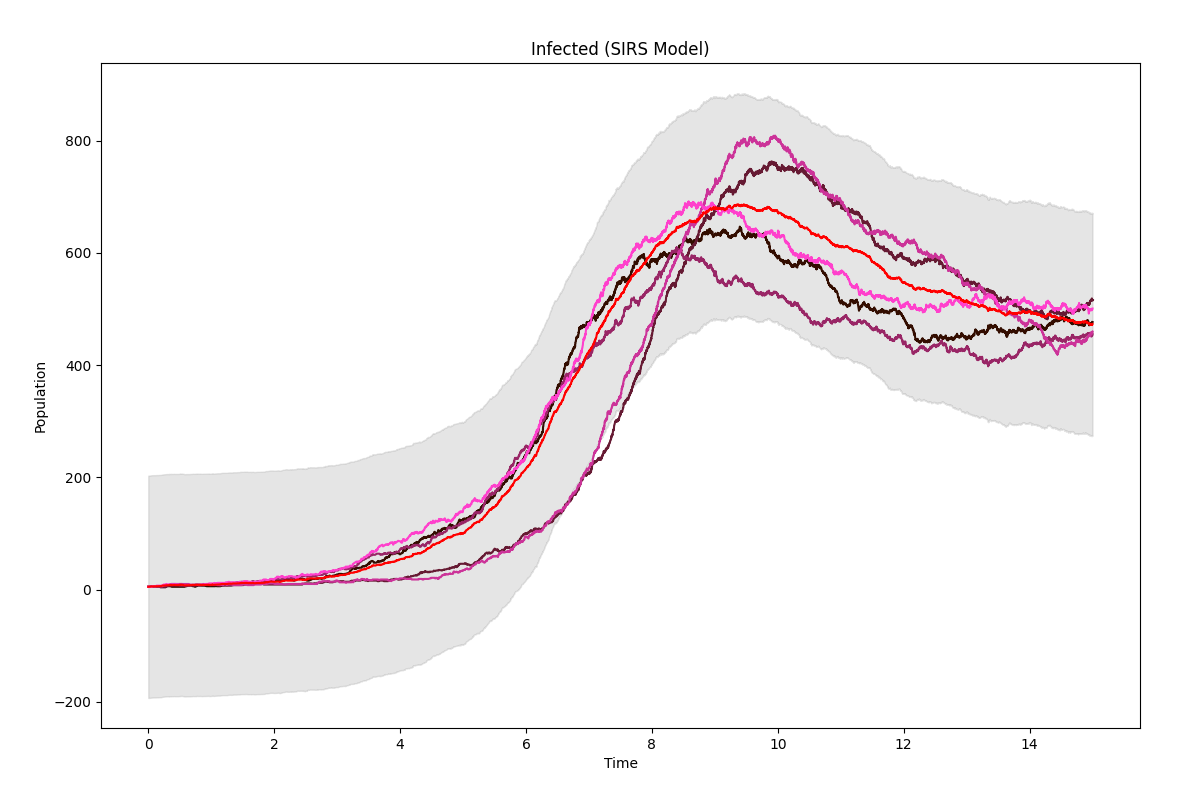
\includegraphics[width=1\textwidth]{Images/Exercise 5/Scenario 1/i1a.png}
        \vspace*{-1cm}
        \caption{Infectados}
        \label{fig:exampleFig16}
    \end{figure}
    
    \begin{figure}[H]
        \centering
        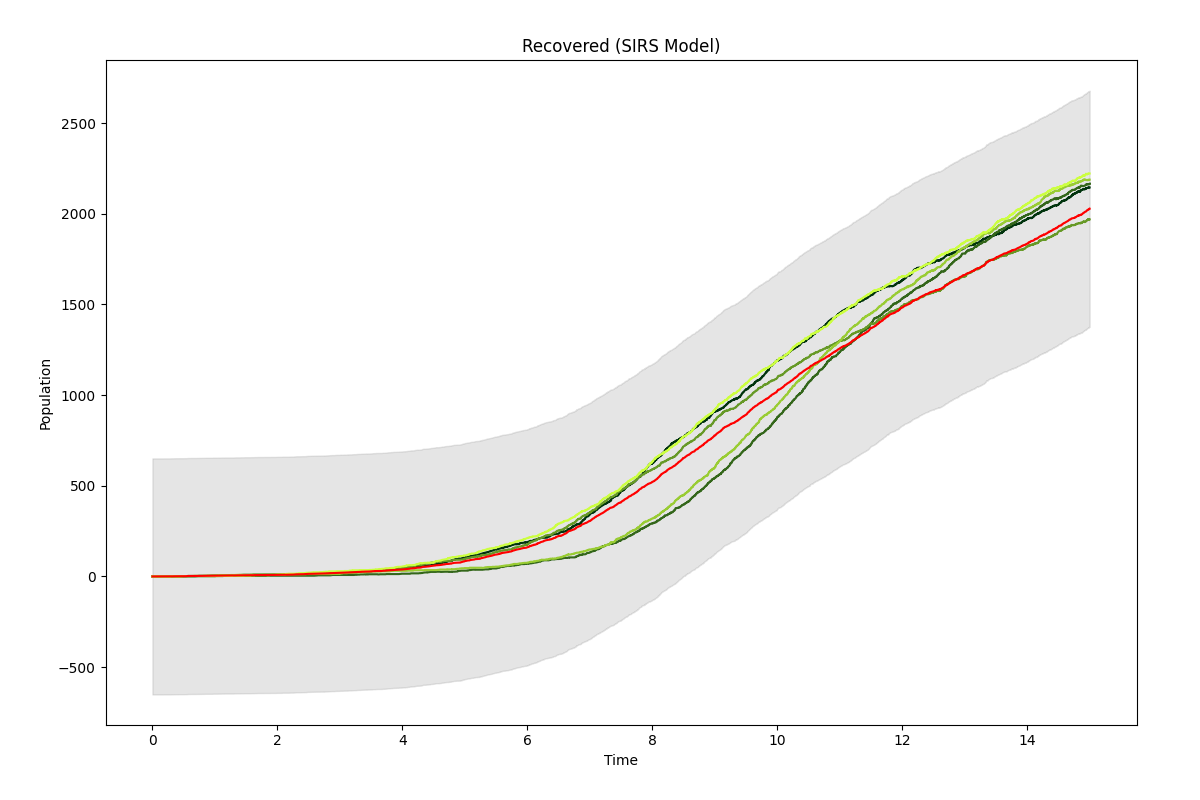
\includegraphics[width=1\textwidth]{Images/Exercise 5/Scenario 1/r1a.png}
        \vspace*{-1cm}
        \caption{Recuperados}
        \label{fig:exampleFig17}
    \end{figure}
    
    \item Segundo Teste
    \begin{figure}[H]
        \centering
        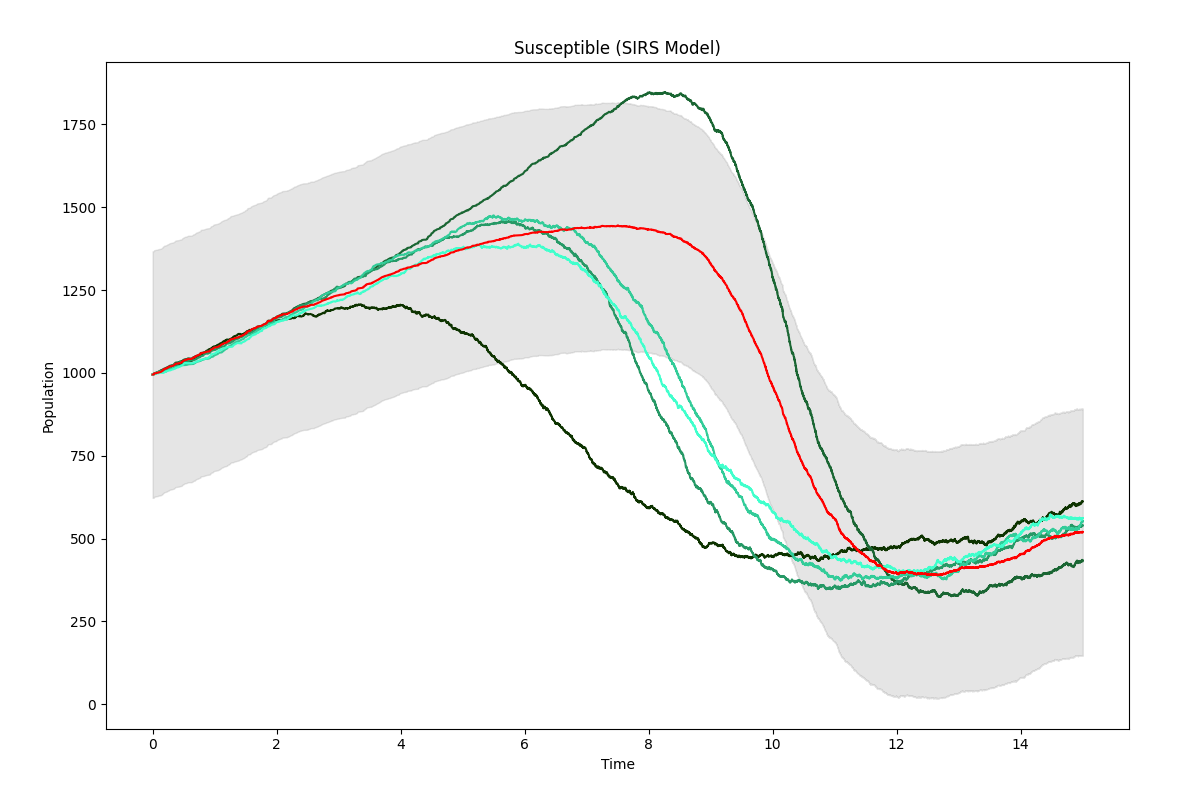
\includegraphics[width=1\textwidth]{Images/Exercise 5/Scenario 1/s1b.png}
        \vspace*{-1cm}
        \caption{Suscetíveis}
        \label{fig:exampleFig18}
    \end{figure}
    
    \begin{figure}[H]
        \centering
        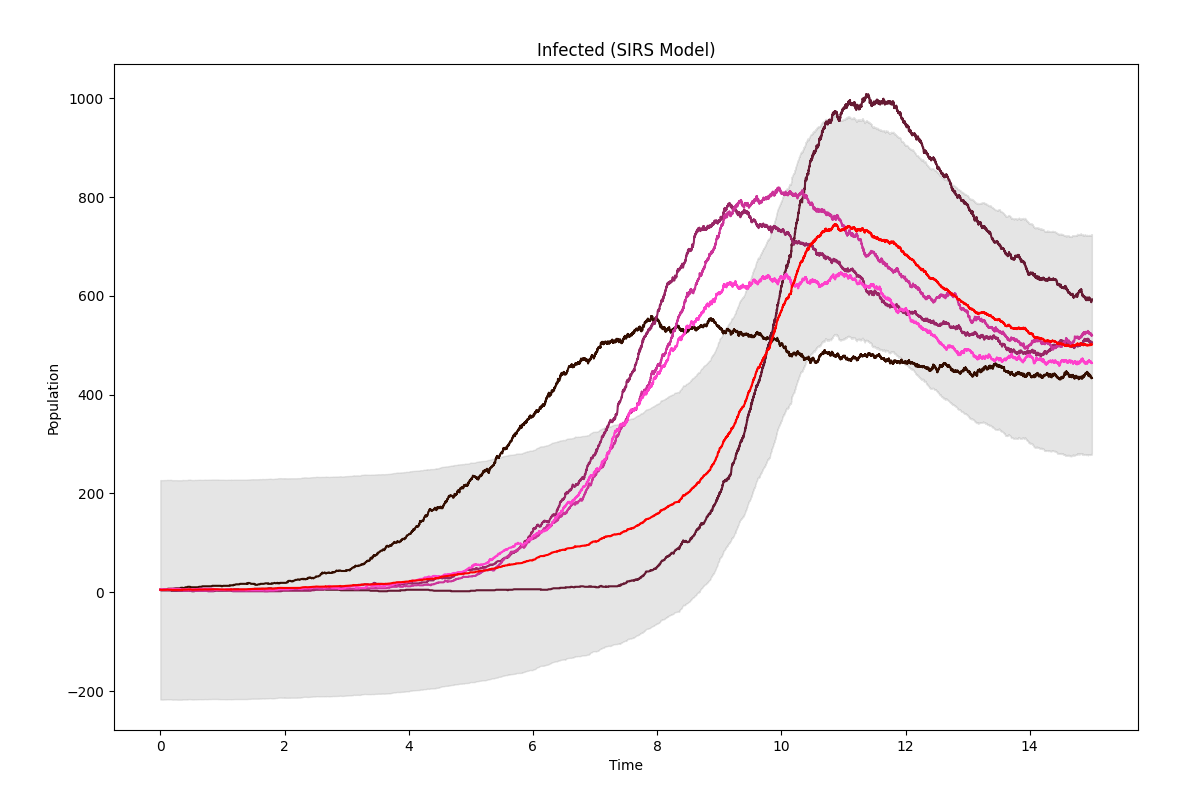
\includegraphics[width=1\textwidth]{Images/Exercise 5/Scenario 1/i1b.png}
        \vspace*{-1cm}
        \caption{Infectados}
        \label{fig:exampleFig19}
    \end{figure}
    
    \begin{figure}[H]
        \centering
        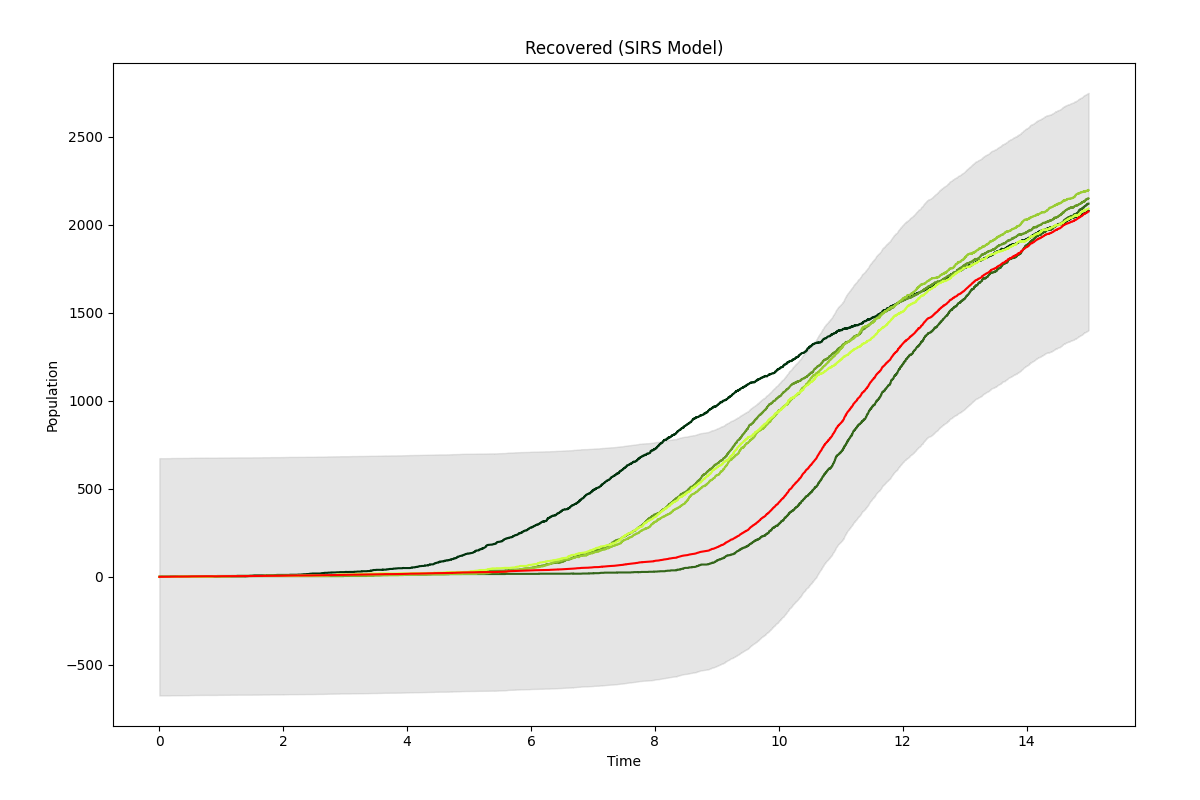
\includegraphics[width=1\textwidth]{Images/Exercise 5/Scenario 1/r1b.png}
        \vspace*{-1cm}
        \caption{Recuperados}
        \label{fig:exampleFig20}
    \end{figure}
\end{itemize}

Entre os dois testes, podemos observar uma dispersão maior no segundo caso, embora a disposição geral das curvas das simulações sejam similares. 

\subsection*{2º Cenário}

Neste segundo cenário, também foram realizados dois testes, cada um executando cinco simulações distintas. Os resultados são sumarizados nas Figuras \ref{fig:exampleFig21}, \ref{fig:exampleFig22} e \ref{fig:exampleFig23}, e \ref{fig:exampleFig24}, \ref{fig:exampleFig25} e \ref{fig:exampleFig26}, respectivamente.

\begin{itemize}
    \item Primeiro Teste
    \begin{figure}[H]
        \centering
        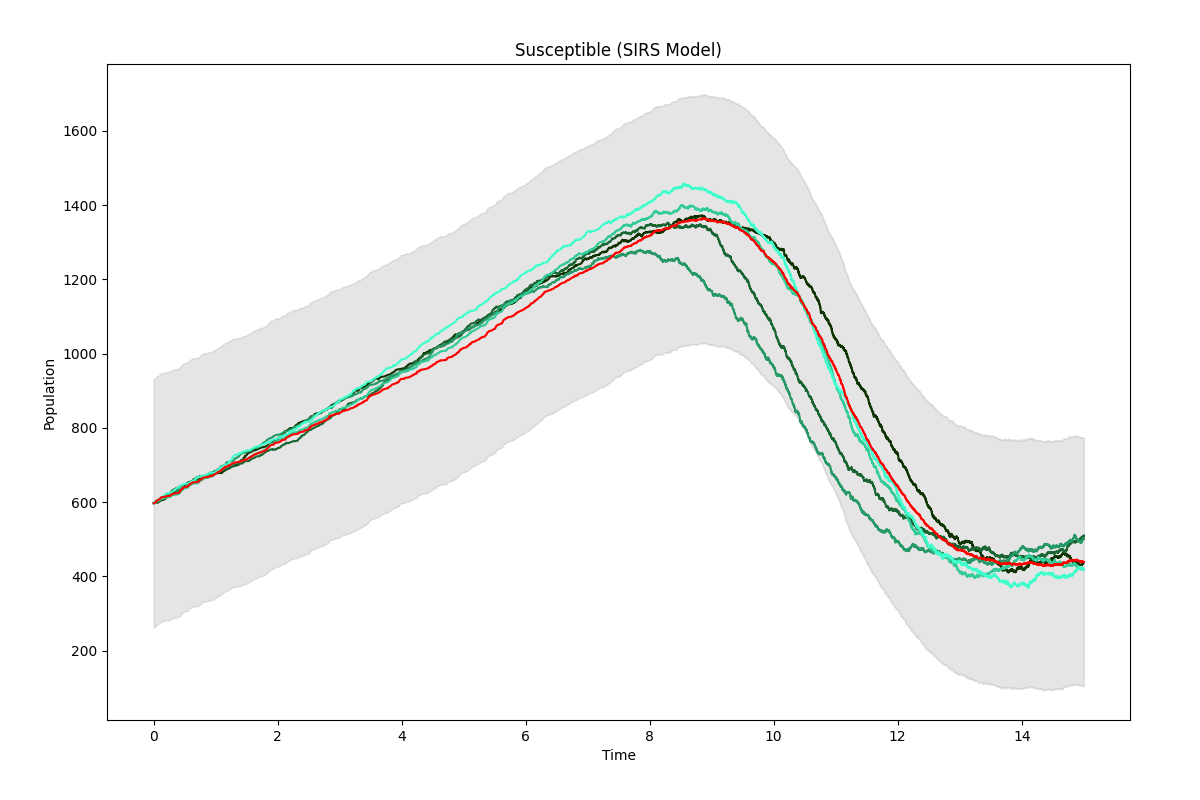
\includegraphics[width=1\textwidth]{Images/Exercise 5/Scenario 2/s2a.png}
        \vspace*{-1cm}
        \caption{Suscetíveis}
        \label{fig:exampleFig21}
    \end{figure}
    
    \begin{figure}[H]
        \centering
        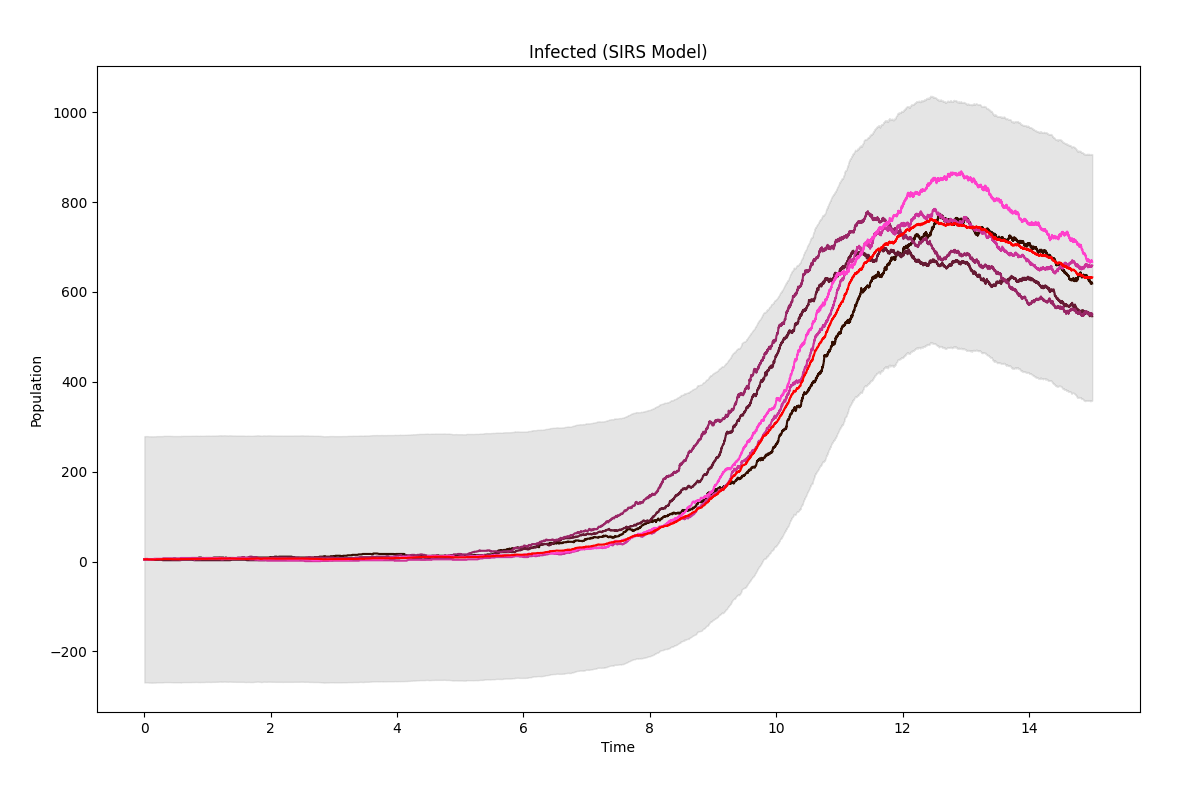
\includegraphics[width=1\textwidth]{Images/Exercise 5/Scenario 2/i2a.png}
        \vspace*{-1cm}
        \caption{Infectados}
        \label{fig:exampleFig22}
    \end{figure}
    
    \begin{figure}[H]
        \centering
        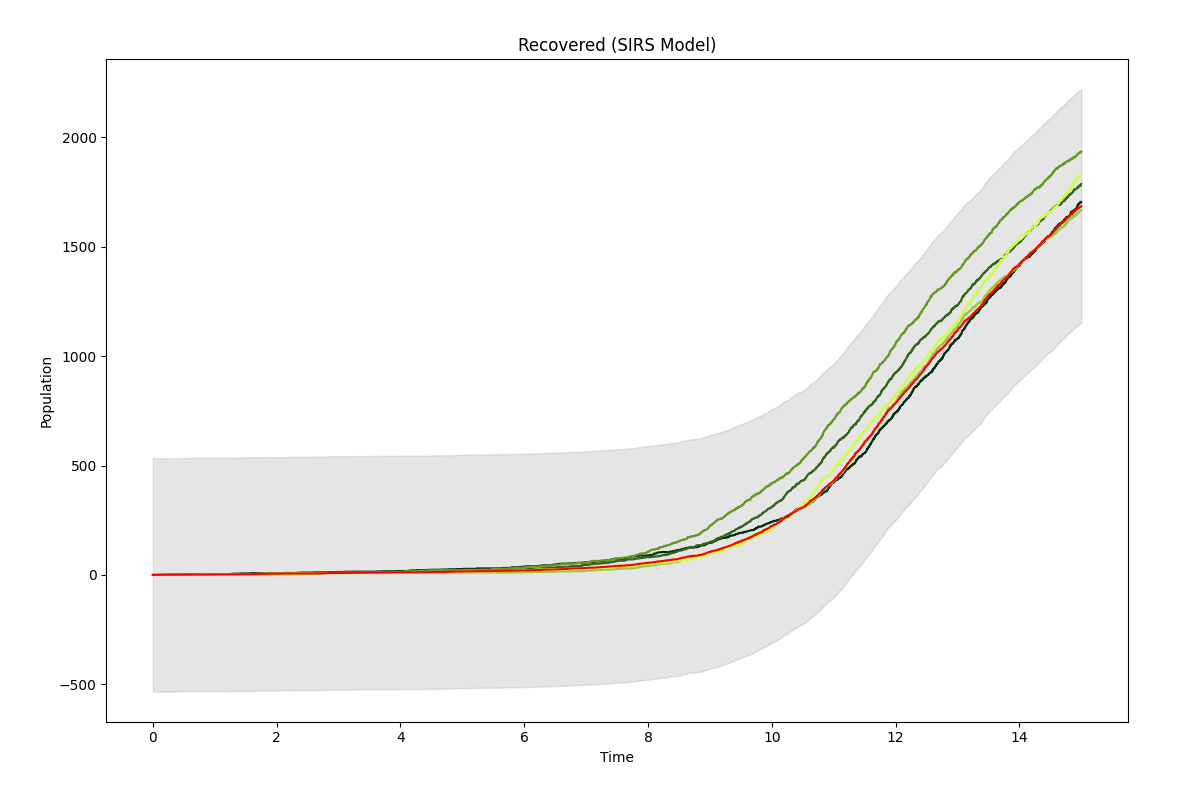
\includegraphics[width=1\textwidth]{Images/Exercise 5/Scenario 2/r2a.png}
        \vspace*{-1cm}
        \caption{Recuperados}
        \label{fig:exampleFig23}
    \end{figure}
    
    \item Segundo Teste
    \begin{figure}[H]
        \centering
        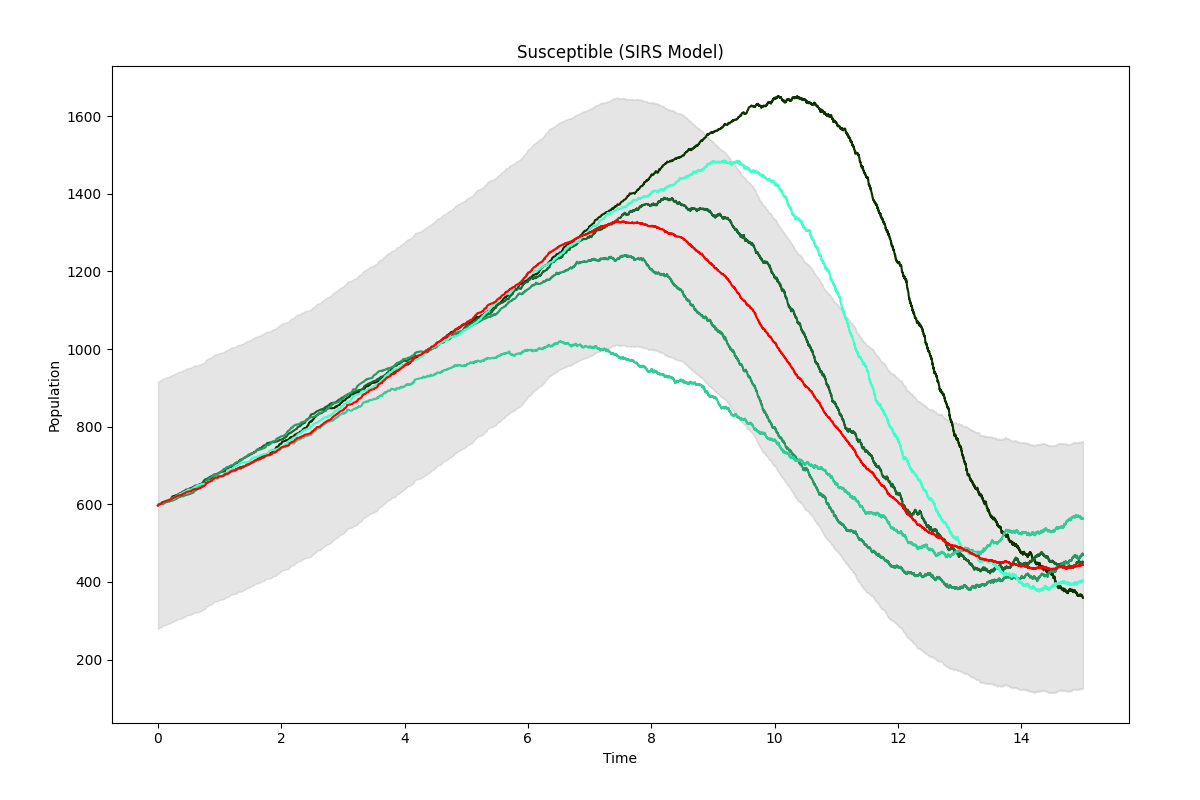
\includegraphics[width=1\textwidth]{Images/Exercise 5/Scenario 2/s2b.png}
        \vspace*{-1cm}
        \caption{Suscetíveis}
        \label{fig:exampleFig24}
    \end{figure}
    
    \begin{figure}[H]
        \centering
        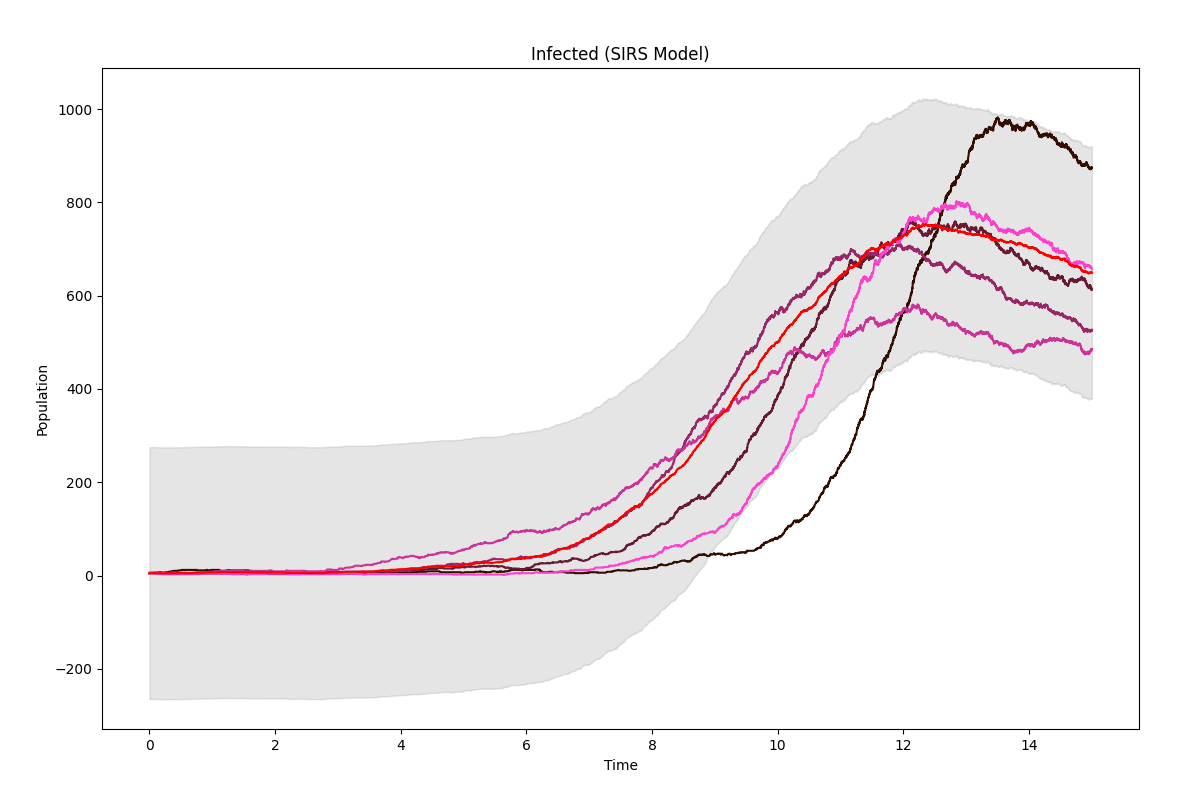
\includegraphics[width=1\textwidth]{Images/Exercise 5/Scenario 2/i2b.png}
        \vspace*{-1cm}
        \caption{Infectados}
        \label{fig:exampleFig25}
    \end{figure}
    
    \begin{figure}[H]
        \centering
        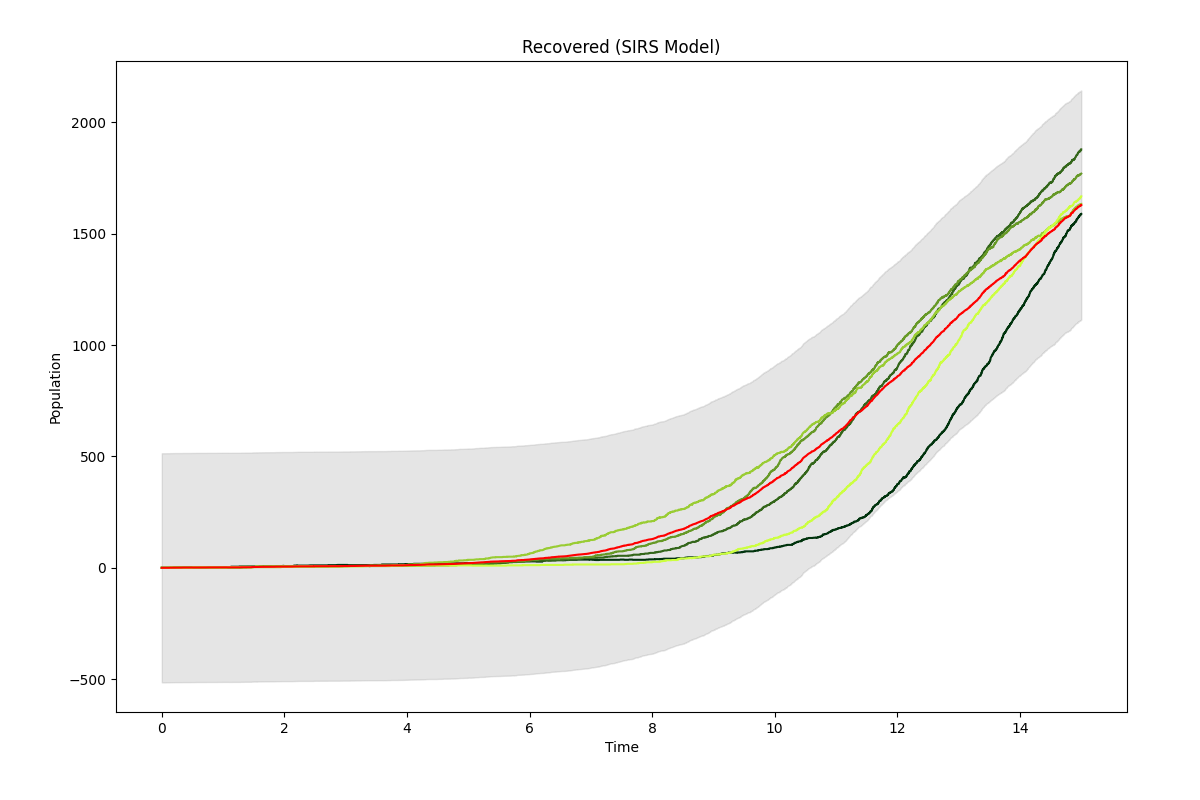
\includegraphics[width=1\textwidth]{Images/Exercise 5/Scenario 2/r2b.png}
        \vspace*{-1cm}
        \caption{Recuperados}
        \label{fig:exampleFig26}
    \end{figure}
\end{itemize}

Novamente, entre os dois testes, podemos observar uma dispersão maior no segundo caso, embora a disposição geral das curvas das simulações sejam similares.

\subsection*{Análise Geral}

Observando o conjunto de simulações, fica evidente que as curvas sem vacinação correspondentes às populações de infectados e recuperados tendem a crescer alguns instantes de tempo mais cedo. Isto porque a população inicial de suscetíveis é quase o dobro do segundo caso.

Outro detalhe interessante, é de que a curva da população de suscetíveis apresenta um leve crescimento logo nos instantes de tempo finais sem vacinação. Quanto maior a texa de vacinação, menos variação e entropia as curvas tendem a apresentar.

Por fim, a aplicação da vacina em instantes de tempo posteriores, provavelmente postergaria o processo de redução da população de suscetíveis e infectados, deslocando as curvas no eixo de tempo.

\pagebreak

\section*{Referências}

\begin{itemize}
    \item Repositório com implementações de métodos e modelos de Alexandre Bittencourt Pigozzo: \url{https://github.com/alexbprr/ComputationalModeling};
    \item Material disponível no portal didático na disciplina de Introdução à Modelagem Computacional.
\end{itemize}

\end{document}
